\section{} \label{tree:bilaga}
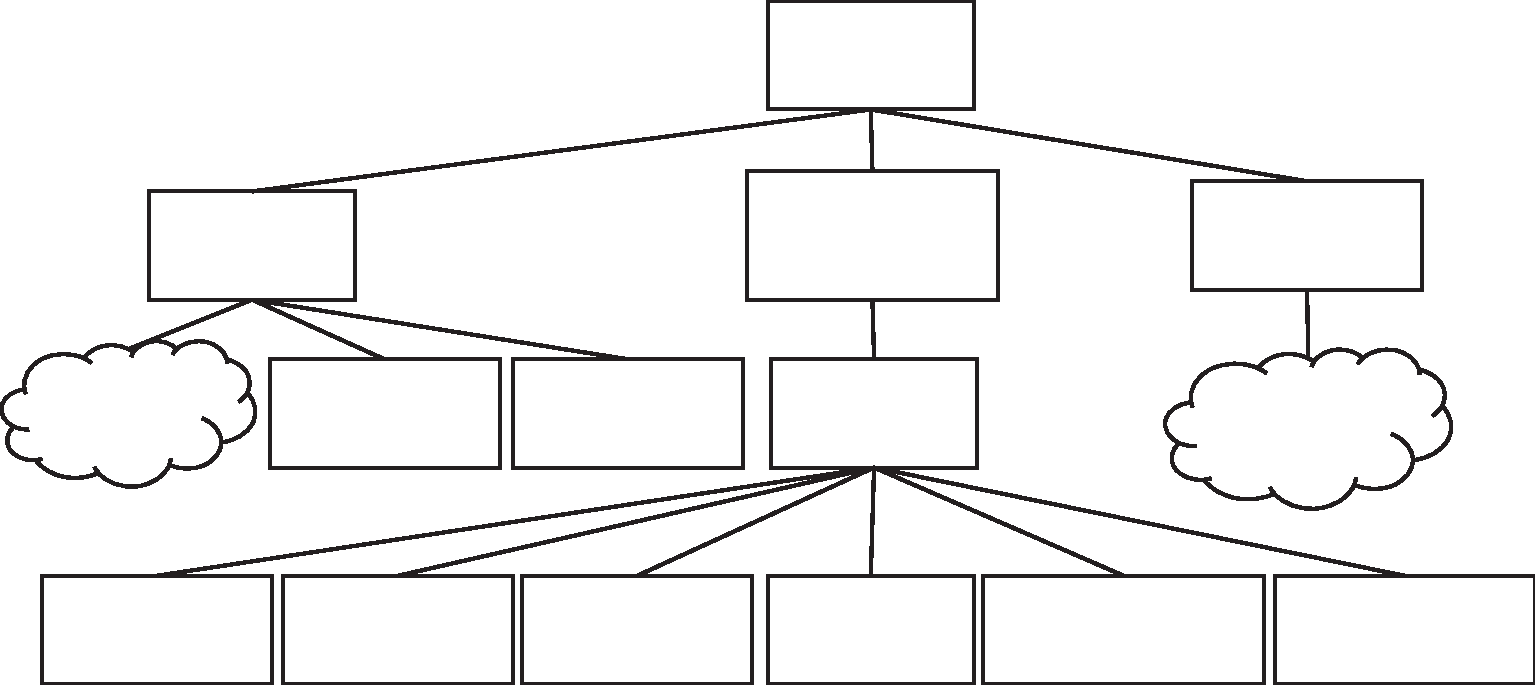
\includegraphics[angle=90,width=8.5 cm]{Bilagor/bilaga-eps-converted-to.pdf}\centering

\section{} \label{hello:bilaga}
\lstset{tabsize=2,breaklines=true,numbers=left,basicstyle=\footnotesize,xleftmargin=30pt}
\lstinputlisting[language=C,]{Kod/helloWorld.c}

% Källkod kan också vara bilaga Källkod, programspråket C inkluderas från filen helloWorld.c som ligger i mappen Kod. Läs  vilka språk som stöds http://en.wikibooks.org/wiki/LaTeX/Source_Code_Listings


% Bilagor hanvisas med \ref{Foretag:koncern} i den löpande texten.
% Exempel: man hänvisa till en bilaga. Se \ref{Foretag:koncern} för mer information.
% kommer att skrivas som:
%m an hanvisa till en bilaga. Se Bilaga A for mer information.

% texten Bilaga A kommer då bli klickbar